\documentclass{article}
\usepackage{tikz}

\renewcommand{\figurename}{Fig.}

\begin{document}

\begin{figure}[ht]
\centering

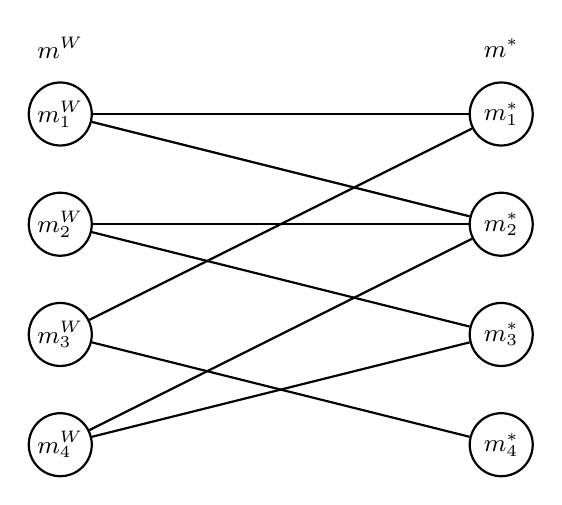
\begin{tikzpicture}[
    x=0.7cm,
    y=0.7cm,
    vertex/.style={
        circle,
        draw,
        thick,
        fill=white,
        minimum size=0.8cm,
        inner sep=0pt,
        font=\small
    },
    partition/.style={
        font=\small
    },
    edge/.style={
        thick
    },
    black edge/.style={
    edge,
    black
    },  
    red edge/.style={
        edge,
        red!70!black
    },
    blue edge/.style={
        edge,
        blue!70!black
    },
    gray edge/.style={
        edge,
        gray!70
    }
]

% Left partition
\node[vertex] (u1) at (0,6) {$m^{W}_1$};
\node[vertex] (u2) at (0,4) {$m^{W}_2$};
\node[vertex] (u3) at (0,2) {$m^{W}_3$};
\node[vertex] (u4) at (0,0) {$m^{W}_4$};

% Right partition
\node[vertex] (v1) at (8,6) {$m^{*}_1$};
\node[vertex] (v2) at (8,4) {$m^{*}_2$};
\node[vertex] (v3) at (8,2) {$m^{*}_3$};
\node[vertex] (v4) at (8,0) {$m^{*}_4$};

% Partition labels
\node[partition] at (0,7.2) {$m^W$};
\node[partition] at (8,7.2) {$m^{*}$};

% Colored edges
\draw[black edge]  (u1) -- (v1);
\draw[black edge] (u1) -- (v2);


\draw[black edge] (u2) -- (v2);
\draw[black edge]  (u2) -- (v3);

\draw[black edge] (u3) -- (v1);
\draw[black edge] (u3) -- (v4);

\draw[black edge]  (u4) -- (v3);
\draw[black edge]  (u4) -- (v2);

\end{tikzpicture}

\caption{A bipartite graph with vertex partitions $m^{*}$ and $m^{W}$.}
\label{fig:bipartite-graph}

\end{figure}

\end{document}